\documentclass[12pt,twoside]{report}
\usepackage[a4paper,width=150mm,top=25mm,bottom=25mm,bindingoffset=6mm]{geometry}
\usepackage[english]{babel}

\setlength{\headheight}{15pt} 

\usepackage[utf8]{inputenc}
%\usepackage[latin1]{inputenc}
\usepackage{fancyhdr}
\usepackage{indentfirst}
\usepackage{graphicx}
\graphicspath{ {Images/}  }
\usepackage{newlfont}
\usepackage{amssymb}
\usepackage{amsmath}
\usepackage{latexsym}
\usepackage{amsthm}
\usepackage{listings}
\usepackage{xcolor}
\usepackage{mdframed}
\usepackage{epigraph}
\usepackage{csquotes}

\usepackage{hyperref}

\usepackage{makecell}
\usepackage{tabularx}
%\usepackage{booktabs}
% \usepackage{graphicx}

\usepackage{tabulary}
\usepackage{epsf} 

\usepackage{breqn}

\usepackage[backend=biber]{biblatex}
\addbibresource{references.bib}

\usepackage{array}
\usepackage{tabu}

\usepackage{amsmath}
\usepackage{amssymb}


\usepackage{lipsum}

%\usepackage{pgf-pie}


%\usepackage{pgfplots}

%\pgfplotsset{
 % compat=newest,
  %xlabel near ticks,
 % ylabel near ticks
%}

\pagestyle{fancy}\addtolength{\headwidth}{20pt}
\renewcommand{\chaptermark}[1]{\markboth{\thechapter.\ #1}{}}
\renewcommand{\sectionmark}[1]{\markright{\thesection \ #1}{}}
\rhead[\fancyplain{}{\bfseries\leftmark}]{\fancyplain{}{\bfseries\thepage}}
\cfoot{}
\linespread{1.3}  
\begin{document}

\begin{titlepage}               

\thispagestyle{empty}                  
\topmargin=6.5cm                        
\raggedleft                            	
\large                                 		
\em                                    
%Questa \`e la \textsc{Dedica}:\\
%ognuno pu\`o scrivere quello che vuole, \\
%anche nulla \ldots     
"Il termine utopia è la maniera più comoda per liquidare quello che non si ha voglia, capacità, o coraggio di fare. Un sogno sembra un sogno fino a quando non si comincia da qualche parte, solo allora diventa un proposito, cioè qualcosa di infinitamente più grande." Adriano Olivetti
\newpage                            
\clearpage{\pagestyle{empty}\cleardoublepage}
\end{titlepage}
\pagenumbering{roman}                   
\chapter*{Abstract}             
\rhead[\fancyplain{}{\bfseries
Abstract}]{\fancyplain{}{\bfseries\thepage}}
\lhead[\fancyplain{}{\bfseries\thepage}]{\fancyplain{}{\bfseries
Abstract}}
Combining smartphone sensors and Internet-of-Things (IoT) enables new kinds of application scenarios. Cowbird is a framework that combines the evaluation of both smartphone sensors and IoT in the cloud. However, Cowbird does not scale well in large deployment contexts where thousands of IoT sensors can continuously generate high volumes of data that have to be processed. To this end, we extended Cowbird to support the sensing and evaluation of large streams of sensor data in real-time. We designed a distributed architecture based on the synergy of traditional computing systems and novel stream data processing technologies. The former is required for building a scalable IoT data sensing platform, while the latter are necessary for evaluating and processing large streams of sensor data. We show that in some conditions the data streams evaluation can be performed directly in the sensing platform. This approach avoids the introduction of extra costs and overheads caused by offloading the sensors data evaluation to a stream data processing engine.




% I made a distributed implementation of the framework that can be executed over many computing nodes. Furthermore, I integrated in the system architecture a real-time stream processing pipeline (using Apache Flink) for evaluating SWAN expressions (queries) over large streams of data generated by IoT sensors

%—Combining sensors from smartphones and Internet
%of Things (IoT) (e.g., light, sound, UV radiation) enables a new kind of -context aware applications in areas like smart cities or smart buildings. Such applications would require continuous evaluation of frequently changing data (smartphone sensors and IoT sensors), and continuous polling of IoT sensor data to the phone. Offloading both the evaluation and the polling of IoT sensor data to the cloud would improve energy efficiency and data transfer costs for the phone. To this end, we built Cowbird, an energy efficient framework to help developers easily build applications that evaluate sensor data both on the phone and in the cloud. To

%%%%%%%%%%%%%%%%%%%%%%%%%%%%%%%%%%%%%%%%%aggiunge la voce Introduzione
                                        %   nell'indice
\addcontentsline{toc}{chapter}{Abstract}
%\input{Introduction}
%%%%%%%%%%%%%%%%%%%%%%%%%%%%%%%%%%%%%%%%%non numera l'ultima pagina sinistra
\clearpage{\pagestyle{empty}\cleardoublepage}

%\rhead[\fancyplain{}{\bfseries\thepage}]{\fancyplain{}{\bfseries
%INDICE}}
\rhead[\fancyplain{}{\bfseries\leftmark}]{\fancyplain{}{\bfseries\thepage}}
\lhead[\fancyplain{}{\bfseries\thepage}]{\fancyplain{}{\bfseries
INDICE}}
\tableofcontents                        %crea l'indice
%%%%%%%%%%%%%%%%%%%%%%%%%%%%%%%%%%%%%%%%%imposta l'intestazione di pagina


%%%%%%%%%%%%%%%%%%%%%%%%%%%%%%%%%%%%%%%%%non numera l'ultima pagina sinistra
\clearpage{\pagestyle{empty}\cleardoublepage}
\listoffigures                          %crea l'elenco delle figure
%%%%%%%%%%%%%%%%%%%%%%%%%%%%%%%%%%%%%%%%%non numera l'ultima pagina sinistra
\clearpage{\pagestyle{empty}\cleardoublepage}
\listoftables                           %crea l'elenco delle tabelle
%%%%%%%%%%%%%%%%%%%%%%%%%%%%%%%%%%%%%%%%%non numera l'ultima pagina sinistra
\clearpage{\pagestyle{empty}\cleardoublepage}
%%%%%%%%%%%%%%%%%%%%%%%%%%%%%%%%%%%%%%%%%imposta l'intestazione di pagina


\lhead[\fancyplain{}{\bfseries\thepage}]{\fancyplain{}{\bfseries\rightmark}}

\pagenumbering{arabic}                  %mette i numeri arabi

\chapter{Introduction}
Modern smartphones are characterized by significant processing power, advanced network capabilities and a variety of different on-board sensing devices such as accelerometer, GPS, gyroscope, ambient light sensors and many others. Mobile applications developers can take advantage of these sensors to build sophisticated applications that affect millions of people lives everyday.

Smartphone sensors create a multitude of opportunities for mobile application developers. Sensed data can be used for building applications such as monitoring the number of steps taken during the day and to remind the user to do physical movement if he/she has been sitting for too long. Sensor-based applications usually collect the data coming from different sensors and use the collected records to provide context-awareness to the end users. However, having many different applications that access the same smartphone sensor can lead to the redundant collection and storage of the same sensor data values. To this extent, the SWAN (Sensing with Android Nodes) framework \cite{swanphd} has been designed. The SWAN framework is a middleware between Android applications and the smartphone sensors. The SWAN framework provides a high-level abstraction to access sensor measurements avoiding data storage duplication. The SWAN framework is characterized by the SWAN-Song language that allows the creation of context expressions based on smartphone sensor data.
%SWAN is integrated with the SWAN-Song domain specific language. The SWAN-Song language lets the mobile application developer to construct high-level context expressions based on smartphone sensors data. Using the SWAN-Song language allows the developers to focus on the logic of the mobile application instead of writing low-level code for fetching and processing data coming from different sensors.

The emergence of the Internet-of-Things (IoT) brings sensors and actuators to the internet. The IoT adoption and deployment contributes to the dissemination of many small sensors over buildings or cities. The combination of smartphone sensors and IoT sensors can enable many new application scenarios. In particular, the local contexts of the user's smartphone can be extended with more global information coming from the surrounding IoT sensors. Hence, applications such as optimizing the biking route through the quietest streets or indicate the most sunny paths can be created. 

%send 
IoT sensors and actuators typically report the sensed data to the cloud. Thus, if a smartphone application wants to access IoT data it has to continuously poll a web endpoint to retrieve the fresh data values. This approach can be very \emph{energy inefficient} for a smartphone. Furthermore, IoT sensors can generate large streams of data that hardly can be aggregated, computed and evaluated by a mobile device. To this end, Cowbird \cite{cowbirdarticle} was created. Cowbird is an energy efficient framework that helps developers build applications that combine smartphone sensor data and IoT. In particular, Cowbird offloads the sensing and communication capabilities to the cloud. Cowbird extends the original SWAN framework making it possible for an Android application to create SWAN-Song expressions that evaluate sensor data both on the phone and in the cloud. 

Internet-of-Things sensors generate continuous streams of data. For example, a smart city with 10,000 sensors (e.g., humidity, sound, CO$_{2}$)  transmitting at a rate of one measurement per second will generate 600,000 data points per minute, or 864 million measurements per day. To address such scenarios, many streaming technologies arose. In such streaming applications, the live data is ingested in a \emph{stream processing engine} that evaluates the data records in real-time. Stream processing frameworks rely on scalable and high-performance computing architectures. 

The current Cowbird cloud application is not designed to scale and it can be executed only on a single computing node. In this thesis, we present an extension of the Cowbird cloud framework designed to sense and evaluate large streams of sensor data in real-time. We organize the Cowbird cloud infrastructure into two layers:
\begin{itemize}
\item A distributed and scalable sensing layer.
\item A high-performance streaming evaluation layer implemented over the Apache Flink processing engine.
\end{itemize}
For some type of SWAN-Song expressions we keep the evaluation in the sensing layer, close to the data generation. This strategy is adopted to avoid communication overheads between the two layers and thus to increase performance. Since the evaluation is performed by a combination of novel streaming technologies and traditional computing systems, we called our architecture \emph{hybrid}. 

\newpage
%\paragraph{}
Our contributions are as follows:
\begin{itemize}
\item We present the design and implementation of a distributed architecture for the Cowbird cloud framework. The architecture is composed of a distributed sensing layer and a streaming evaluation layer powered by a streaming engine. 

\item We implement an optimized evaluation strategy for the SWAN-Song expressions that can be used in streaming-oriented applications.

\item We build an experimental application that makes usage of sound sensors. We use this application to test and evaluate our proposed Cowbird cloud architecture. We also describe a benchmark framework we built for evaluating stream processing engines. The framework helped us understanding which streaming engine among all the available platforms is the most suitable for our use case.

\end{itemize}

\paragraph{}
This thesis is structured as follows: 
\begin{itemize}
\item \textbf{Chapter 2} provides background information about the SWAN framework and Cowbird.
\item	 \textbf{Chapter 3} describes the large-scale architectures that can be used to analyze streams of data in real-time.
\item \textbf{Chapter 4} gives an overview of the cutting-edge stream processing technologies. In this chapter, we also describe the framework we built for evaluating some of the available stream processing engines.
\item \textbf{Chapter 5} describes the design and implementation details of the extend Cowbird architecture.
\item \textbf{Chapter 6} reports the testing methodologies adopted and the evaluation results of the proposed distributed architecture.
\item \textbf{Chapter 7} reports the related work in streaming architectures applied to the IoT scenarios. 
\end{itemize}

\clearpage{\pagestyle{empty}\cleardoublepage}
\chapter{Background}

In this chapter we present the existing Cowbird framework described within the SWAN project \cite{swanonline}. Cowbird is a flexible and energy efficient framework for building Android applications that use both smartphone sensors and IoT sensors\cite{cowbirdarticle}. Cowbird extends the SWAN framework \cite{swanphd} and it supports context-based expressions (queries) that can run both on a smartphone and in the cloud; with the Cowbird framework, developers can easily decide where to perform the computation according to the source of the data and the frequency of the updates.

\section{The SWAN Framework}
SWAN (Sensing With Android Nodes) is a framework for easily building context-aware applications for Android smartphones \cite{swanphd}. The framework provides application developers a high-level abstraction for accessing smartphone's sensors. In particular, the SWAN framework is designed to be executed as an Android background service and it acts as a middleware between applications and sensors: running applications can access it through a well-defined API. The SWAN framework reduces storage redundancy and code duplication caused by multiple sensor-based applications running simultaneously. In fact, it provides a centralized solution for collecting and storing data from sensors. 

\subsection{SWAN Sensors}
One of the most important characteristic of SWAN is its \emph{multi sensor support}; at the moment, SWAN supports more than 20 different types of sensors. Below, we describe two categories of sensors:
\begin{itemize}
\item	 \emph{Hardware sensors}. The physical sensors installed on the devices (e.g. accelerometer, GPS).
\item \emph{Software sensors}. Software \emph{data sources} (e.g., calendar, rain prediction, Twitter) that can be installed on the devices or that can run somewhere else. 
\end{itemize}

SWAN sensors are implemented as background services that are responsible for gathering the sensor's data. In case of external software sensors such as the rain prediction or Twitter, the SWAN sensor continuously polls from the web endpoint to get live data. The data accuracy can be improved by increasing the polling frequency. 

From an architectural point of view all the SWAN sensors run in separate processes in order to remain unaffected if the application built on top of SWAN crashes: this design approach prevents data losses. The communication between SWAN sensors and the other components is performed through inter-process communication (IPC).

\subsection{SWAN-Song}
SWAN-Song \cite{swansong} is a domain specific language
for context expressions. SWAN-Song is used by applications to register expressions into SWAN. After registering an expression, SWAN evaluates it and sends back the result to the application. 

The SWAN-Song language is a form of zeroth-order logic, which allows the description of a particular combination of contextual information using sensor based expression predicates. The predicates can be combined using math, comparison, and logic operators, and a specification of a \emph{history window} and \emph{history reduction} operator.  

\subsubsection{SWAN-Song Expressions \& Predicates}
A SWAN-Song expression is composed of two required components and three optional components. The required components are a sensor entity and a value path. The optional components are a list of one or more configuration parameters, a history window and a history reduction mode.

There are two types of SWAN expressions:
\begin{itemize}
\item \emph{Value expressions}. Such expressions return a sensor value or a list of sensor
values. For example, the following expression gets the current light intensity:
\begin{equation} \label{eq:luxexpression}
self@light:lux\big\{MEAN, 2000ms\big\}
\end{equation}
In expression (\ref{eq:luxexpression}) \emph{self} is the location identifier of the device, light
is the sensor name, \emph{lux} is the value path, \emph{MEAN} represents the history reduction mode and \emph{2000ms} indicates the history window. The expression computes the average value generated by the light sensor in the last 2000 milliseconds.

\item \emph{Tristate expressions} Such expressions are useful for defining complex context conditions and they can take one of the following values: TRUE, FALSE or UNDEFINED. An expression is evaluated to UNDEFINED if the sensor queried in the expression is turned off or not available. As an example, the following expression(s) can be used to notify the user that he/she should exercise:
\begin{equation} \label{eq:morningexpression}
Morning = self@time:hour < 12 
\end{equation}
\begin{equation} \label{eq:dryexpression}
Dry = self@rain:expected == 0 
\end{equation}
\begin{equation} \label{eq:mobilityexpression}
Mobility = self@movement:total \big\{MAX,3600000\big\} > 15.0
\end{equation}
\begin{equation} \label{eq:exerciseexpression}
Exercise = Morning \text{ \&\& } Dry \text{ \&\& }  \text{!} (Mobility)
\end{equation}
\end{itemize}
The \emph{Morning} expression (\ref{eq:morningexpression}) uses the time sensor to
check if it is earlier than 12:00 pm; the \emph{Dry} expression (\ref{eq:dryexpression}), instead, checks the live rain prediction using the rain sensor and \emph{Mobility} (\ref{eq:mobilityexpression}) uses the accelerometer sensor to check if the user has been moving in the past hour. The \emph{Exercise} expression (\ref{eq:exerciseexpression}) combines the other TriState expressions to determine whether or not the context of the user is suitable for a workout.

Sensor predicates represent an array of \emph{time-stamped values} because of the time windowing of sensor values. History operators are then applied on these values collected within the time specified time frame. SWAN-Song expressions support different history reduction modes, such as:
\begin{itemize}
\item ALL. This operator checks if \emph{all} the time-stamped values, sensed within the time window, match the condition defined in the SWAN-Song expression.
\item ANY. Selects any value that makes the comparison \emph{true} as the value of the sensor. The ANY operator is also the default history reduction mode.
\item MIN, MAX, MEAN, and MEDIAN, which will select or calculate the appropriate value.
\end{itemize}

\subsection{Architecture}
Android applications can register SWAN-Song expressions using the SWAN API. On registering a new expression, the Expression Evaluation Engine (see Figure \ref{fig:cowbird_architecture}) is invoked. The Expression Evaluation Engine is responsible for evaluating SWAN-Song expressions: it interacts with the sensors in order to fetch the sensed data and computes the result of the expressions. Whenever new sensed data is available, it is sent to the Expression Evaluation Engine, which processes it and sends the result back to the application.

 \begin{figure}[ht!]
\includegraphics[width=1\textwidth]{images/cowbird_architecture.png}
 \caption{SWAN and Cowbird architecture. Cowbirds components are marked with $\otimes$. Source: \cite{cowbirdarticle}}
\label{fig:cowbird_architecture}
\end{figure}

\section{The Cowbird Framework}
The Cowbird framework has been designed as a cloud extension of the SWAN framework. In particular, it enables the combination of smartphone sensors and real-time web data: these data can be originally generated by IoT sensors or any data which can be retrieved by polling a web resource (e.g. Twitter feeds) \cite{cowbirdarticle}. Furthermore, the Cowbird framework reduces the overall communication between the smartphone and the cloud in order to save energy. In fact, the evaluation of phone sensors is performed locally while the evaluation of IoT sensors is computed in the cloud.


The description below has been adapted from \cite{cowbirdarticle} and contains textual overlap with the paper. Some of the core features and characteristics of Cowbird are \cite{cowbirdarticle}:
\begin{itemize}
\item \emph{Flexibility}. The developers using the Cowbird framework
can easily connect to any cloud to offload the evaluation of the IoT sensors.
\item \emph{Usability}. Cowbird uses the SWAN-Song domain specific language to access both sensors in the phone and real-time data.
\item \emph{Portability}. The cloud part of Cowbird is programmed in
Java. Hence, it can be easily ported to any device running a JVM.
\item \emph{Privacy}. Cowbird performs the evaluation of local sensors
on the phone and evaluation of remote IoT sensors remotely. Thus, the sensitive data can be kept and processed locally on the phone.
\item \emph{Energy Efficiency}. Cowbird is designed to minimize the energy consumption of smartphones. Offloading the computation and the communication required to fetch the IoT real-time data (continuous polling from the web) to the cloud will preserve the smartphones battery life.
\item \emph{Mobile Data Cost}. Sending much data through cellular
networks is costly, so Cowbird tries to optimize the communication between the phone and the cloud. The result of the evaluation in the cloud is only sent to the phone if there is a change from the previous result. 
\end{itemize}
\subsection{Cowbird Architecture Details}
Cowbird enriches the SWAN framework designed to be executed on Android smartphones. In particular, Cowbird integrates novel capabilities to the existing SWAN services and it introduces new sensing services to be executed on the cloud. 

The existing SWAN framework has been extended by modifying the SWAN-Song language in order to support \emph{cloud-based expressions}. Furthermore, a new module named \emph{Cloud Manager} has been introduced: it runs on the smartphone and it is responsible for managing the communication with one or more clouds \cite{cowbirdarticle}. 

At the cloud side, the original SWAN evaluation engine has been redesigned to be executed on the cloud. The cloud side of the framework has support for various IoT sensors (implemented as virtual sensors and executed by a different thread) and a mechanism to push data to the phone.

\paragraph{}
We discuss now the typical interaction flow between Cowbird and  third-party app built on top of it. A third-party app uses the SWAN API to register a remote expression to the cloud. The expression is then sent to the evaluation engine service which will forward it to the cloud manager in the phone. The cloud manager checks the location identifier of the expression and sends it to the specified URL. The cloud acknowledges the expression and starts the evaluation by activating the relevant sensor thread. The result of the evaluation from the cloud is received by the cloud manager and is further sent to the evaluation engine in the phone for local processing. The final result is then sent back to the app.

\subsubsection{Remote Expressions in Cowbird}
%	configuration app of the framework
In Cowbird, the location identifier of SWAN-Song has been extended in order to support remote expressions. The developer can add the URL of its cloud in the configuration of the SWAN framework. The developer can then refer to that cloud using \emph{cloud} as location identifier in its SWAN-Song expression. For example, in case of a sound sensor feed available in a certain channel of the ThingSpeak platform \cite{thingspeakonline} we can write a SWAN expression such as:
\begin{equation} \label{eq:cloudthingspeakexpression}
cloud@thingspeak:field?channelid='1'\#field='1'\big\{MEAN,20s\big\} > 50.0
\end{equation}
The expression \ref{eq:cloudthingspeakexpression} checks if the mean value over a period of 20 seconds is greater than 50.0 decibel (dB). 

The developer can also refers to the cloud indicating the endpoint directly in the SWAN-Song expression. For example, the following SWAN-Song expression perform the same evaluation of expression \ref{eq:cloudthingspeakexpression}:
\begin{equation} \label{eq:herokuthingspeakexpressionurl}
url=http://cowbird.herokuapp.com
\end{equation}
\begin{equation} \label{eq:herokuthingspeakexpression}
url@thingspeak: field?channelid='1'\#field='1'\big\{MEAN,20s\big\} > 50.0
\end{equation}
The SWAN-Song expression \ref{eq:herokuthingspeakexpression} assumes to have a Cowbird cloud instance running on Heroku at the URL provided as location identifier of the expression.

A combination of expressions that use smartphone local sensors (accelerometer) and IoT sensors (live data coming from ThingSpeak) can be written as:
\begin{equation}
E1 = self@movement:total\big\{ANY,1000\big\} > 15 
\end{equation}
\begin{equation}
E2 = cloud@thingspeak:field?channelid='1'\#field='1'\big\{MEAN,20s\big\} > 50.0
\end{equation}
\begin{equation} \label{eq:localcombinedexpression}
CombinedExpression = E1 \text{ \&\& } E2
\end{equation}
The evaluation of the local expression (E1) occurs locally on the Android smartphone. The evaluation of the remote expression (E2) occurs in the cloud and the result is sent to the phone. The CombinedExpression in \ref{eq:localcombinedexpression} is evaluated on the phone based on the results from E1 and E2. 

The evaluation of a SWAN-Song expression composed by two remote sub-expressions, instead, is completely evaluated in the cloud.
\begin{equation}
E1 = cloud@thingspeak:field?channelid='1' \#field='1'\big\{MEAN,200s\big\} > 50.0
\end{equation}
\begin{equation}
E2 = cloud@thingspeak:field?channelid='2' \#field='1'\big\{MEAN,200s\big\} > 50.0
\end{equation}
\begin{equation} \label{eq:remotecombinedexpression}
CombinedExpression = E1 \text{ \&\& } E2
\end{equation}

The result of the combined expression in \ref{eq:remotecombinedexpression} is evaluated on the cloud; the combined result is then sent to the phone.
\subsubsection{Cloud Manager}
The description below has been adapted from \cite{cowbirdarticle} and contains textual overlap with the paper. The evaluation engine running on the smartphone registers an expression to the cloud manager using three parameters: the expression identifier, the expression itself and the location (URL) of the expression. The cloud manager makes a HTTP POST request to the cloud indicated by the expression with the id, expression and a Firebase token. The cloud manager runs a Firebase Message Service used to receive the result of the evaluation computed in the cloud. The result is received at the smartphone side as push notification through Firebase Cloud Messaging. 
% We chose Firebase Cloud Messaging because sensor data is typically less than 4KB (maximum payload). 
Since Cowbird is Android-based, the Google Play Service already has socket connections to the Firebase server and multiple applications can use this service to minimize battery consumption. The message received from the server contains the result of the expression which can be either a new value or a new TriState (TRUE, FALSE, UNDEFINED) and the expression id. The Cloud manager sends this data to the evaluation engine service for local evaluation. After the local evaluation, the final result is sent to the app.
\subsubsection{Cloud Instance}
The description below has been adapted from \cite{cowbirdarticle} and contains textual overlap with the paper. The Cowbird cloud instance is implemented using the Play Framework \cite{playframeworkonline} with Java. The Cloud API contains a controller that routes a specific URL to a functionality. The cloud instance supports requests to register expressions both from mobile clients and web clients. The Cowbird cloud instance currently supports various IoT sensors such as ThingSpeak, The Things Network, Twitter, News, Weather, Currency and Flight. Additional sensors can be easily added as a plugin. Sensors are implemented as Java threads.

 \begin{figure}[ht!]
\includegraphics[width=1\textwidth]{images/cowbird_communication.pdf}
 \caption{SWAN smartphone and Cowbird communication architecture.}
\label{fig:cowbird_communication_architecture}
\end{figure}

On receiving a request from the phone, the Cloud API forwards it to the evaluation engine. The evaluation engine will start the relevant sensor thread that will keep polling external web data from an endpoint. The sensor data is sent back to the evaluation engine which will evaluate the data;  expression evaluation performed in a multi-threaded fashion. The evaluation result is sent to the Cloud API that will forward it to the phone.
%along with the registered token and the framework’s API key \cite{cowbirdarticle}
The communication between the Cowbird cloud instance and the phone happens through Firebase push notification (see Figure \ref{fig:cowbird_communication_architecture}).
\subsection{Optimization}
The process of sending back from the Cowbird cloud instance to the smartphone the result of a SWAN-Song Tristate expression has been optimized. The result is sent back only if there is a change in the evaluation (e.g., from FALSE to TRUE) and not every time a sensor value changes \cite{cowbirdarticle}. Minimizing the communication between the phone and the cloud reduces the energy consumption and preserves the smartphone battery life.
\section{Cowbird Limitations}
The Cowbird architecture presents some limitations. In particular, the current implementation of the cloud instance does not scale since it is designed to run on a single computing node. Now imagine a scenario where many expressions from different smartphones are offloaded to the cloud; thus, many threads are instantiated in order to fetch the sensor data. Multiple running threads can easily saturate the computing resources especially if each thread performs updates with a high frequency. Furthermore, each sensor generates an unbounded and potentially infinite stream of data that has to be processed by the evaluation engine. The huge amount of data that has to be processed can overwhelm the computing resources (i.e. CPU, memory) and reduce the overall performance of the framework.

In order to evaluate the streams of data generated by the IoT sensors in real-time a distributed computing architecture is required. In the next chapters we will investigate how such infrastructure can be built and how the Cowbird cloud instance can be extended. We will focus on how Cowbird can accommodate SWAN-Song expressions evaluation on a large scale.
\clearpage{\pagestyle{empty}\cleardoublepage}
\include{architecture}
\clearpage{\pagestyle{empty}\cleardoublepage}
\chapter{Stream processing frameworks}
In the previous chapter, we have seen that the crucial component of a large-scale streaming infrastructure is a low latency stream processing engine. The big data streaming landscape is constantly growing and many distributed stream processing frameworks are available today. Since we want to extend 
the current Cowbird framework in a way it can support the processing of large amount of data in real-time, we extensively studied and analyzed some of the stream processing frameworks currently available. We also build a small benchmark framework that helped us understanding which engine is the most suitable for our use case.

In this chapter, we will discuss the architectural characteristics and main features of the cutting-edge stream processing technologies. Finally, we will describe the benchmark framework we built for evaluating some of these streaming engines.
\section{Overview}
Sensors monitoring, network traffic analysis and security threats detection are some of the applications that generate large amount of data to be processed in real-time. These stream applications are characterized by an unbounded sequence of events that continuously arrive and need to be processed with a relative low latency. The advent of the Internet-of-Things (IoT) increases the need of real-time monitoring \cite{streamprocessingcomparison}. In fact, Gartner Inc. forecasts that more than 8 billion connected things will be in use worldwide in 2017 and will reach 20.4 billion by 2020 \cite{gartnerarticleonline}. Hence, the amount of data generated cannot always be processed centrally. A distributed architecture is desired in order to process such volume of data.  In these systems, the input data is partitioned and treated in parallel. Thus, high availability and fail recovery are critical in stream processing systems. The stream processing platforms must provide resilience mechanisms against faults, such as delays, data loss, or out of order samples, which are common in data stream. In low latency applications, the recovery should be quick and efficient, providing processing guarantees \cite{streamprocessingcomparison}. Streaming frameworks usually support one or more of the following processing guarantee semantics:
\begin{itemize}
\item \emph{At-most-once}. Each input sample or message is processed at most one time. In case of failures, the sample/message is not reprocessed.
\item \emph{At-least-once}.  Each input sample or message is processed at lest one time. In case of failures, the sample/message might be reprocessed multiple times and multiple results are delivered.
\item  \emph{Exactly-once}. Each input sample or message is processed once and only once.
\end{itemize}

Stream processing systems have a highly optimized execution engine to provide real-time response for applications with high data-rates. In order to achieve a good processing performance and keeping latency within microseconds streaming platforms minimize communication overheads when data trasmission is required between distributed computations \cite{streamprocessingcomparison}. There are two methods of data processing in streaming processing systems \cite{streamprocessingcomparison}:
\begin{itemize}
\item \emph{Micro-batch processing}. Micro-batch treats the stream as a sequence of smaller data blocks. For small time intervals, the input is grouped into data blocks and delivered to a traditional batch system to be processed.
\item \emph{Stream processing}. The stream processing analyzes and processes massive sequence of unlimited data that are continuously generated. In contrast to micro-batch, it is not limited by any unnatural abstraction.
\end{itemize}

Micro-batch engines have a higher latency in comparison to pure stream processing engines. However, fault tolerance and load balancing are much more efficient in micro-batch processors since, in case of failure, the (micro) batch assigned to the failing node can simply be reappointed to another available machine. Viceversa, in pure streaming engines, fault tolerance is performed for each processed message introducing extra overheads.

As already mentioned, the streaming technologies landscape is very rich and there are many streaming engines available. In the following sections, we will briefly discuss the cutting-edge stream processing technologies available right now.

\section{Apache Storm}
One of the most established streaming engine is Apache Storm \cite{apachestormonline}. It was originally designed at BackType and then open sourced after being acquired by Twitter. This system has a pure streaming process engine with a very low latency. However, Storm has also a low throughput and at-least-once processing semantics. In order to add exactly-once semantics to Storm, Twitter created Trident: 
it provides a high-level abstraction on top of Storm that brings exactly-once semantics and \emph{stateful} stream processing (the engine keeps an internal state of the data is being processed) to the platform. This is made possible since Trident treats pure streams of data as sequences of micro-batches. Micro-batch incurs to extra latency, even tough it increments the throughput. In reaction to these issues, Twitter in 2015 announced Heron \cite{herononline}. Heron was developed internally at Twitter and it provides low latency and high throughput but it has support only for at-least-once and at-most-once processing semantics \cite{streaming@twitter, heron}. 
\section{Apache Samza}
Apache Samza \cite{apachesamzaonline} is an open-source stream processing framework originally developed in conjunction with Kafka at LinkedIn \cite{philosophydistributeddata}. In fact, a Samza job consists of a Kafka consumer, an event loop that calls the application code to process incoming messages, and a Kafka producer that sends output messages back to Kafka \cite{philosophydistributeddata}. For each partition of an input topic of a Samza job, a computing unit named StreamTask is allocated. Each task instance consumes messages from just one partition; the task instances can run on the same node or they can be distributed across multiple machines. In Apache Samza, fault tolerance is guaranteed by Kafka. Samza does not implement its own network protocol for transporting messages from one operator to another; in fact, all the communications between computing nodes depend on Kafka \cite{philosophydistributeddata}. Since Apache Samza highly relies on Kafka, it is considered a full-streaming processing engine. However, it also supports batch processing \cite{philosophydistributeddata}. Kafka initially supported only at-least-once semantics, thus Samza has the same degree of processing guarantee. However, Confluent, the company behind Kafka, recently announced the introduction of exactly-once semantics in Apache Kafka in its 0.11 release.

Samza implements durable state within streams of data using a key-value store abstraction. In particular, Samza uses the RocksDB \cite{rocksdbonline} embedded key-value store, which provides low-latency and high-throughput access to data on local disk \cite{philosophydistributeddata}. 

\section{Apache Spark Streaming}
Apache Spark Streaming \cite{apachesparkstreamingonline} extends the Apache Spark framework introducing the discretized streams (D-Streams) programming model \cite{apachesparkstreaming}. The key idea behind D-Streams is to treat a streaming computation as a series of deterministic batch computations on small time intervals or windows. A discretized stream is just a series of RDDs  grouped together; this series of RDDs contains data arrived within a certain time interval. D-Streams provide both \emph{stateless} operators which act independently on each time interval, and \emph{stateful operators}, such as aggregation over a defined sliding window, which operate on multiple intervals and may produce intermediate RDDs as stream state. Spark Streaming takes care of distributing the state in the cluster, managing it, transparently recovering from failures, and providing fault tolerance.

Fault tolerance is guaranteed in Spark Streaming in the same way it is implemented in Spark; a (micro) batch is simply reassigned to another available node in case of failure. In particular, D-Streams use an approach called \emph{parallel recovery}. The system periodically checkpoints RDDs state, by asynchronously replicating them to other nodes. When a node fails, the system detects the missing RDD partitions and launches tasks to recover them from the latest available checkpoint. Multiple fine-grained tasks can be launched concurrently in order to compute different RDD partitions on different nodes \cite{apachesparkstreaming}. 

Spark Streaming supports exactly-once sematincs, it has a very high throughput but also a notably latency because of its micro-batching engine \cite{streamprocessingcomparison, yahoobenchmarkingonline, zalandobenchmarkingonline}. 

Spark Streaming supports also full batch processing, making possible the combination of the two approaches. 

\section{Apache Flink}
Apache Flink \cite{apacheflinkonline} is an open-source stream processing framework. It is a full stream processing engine and it is based  on its majority on the Google’s Dataflow Model \cite{googledataflow}. Flink supports also a full-fledged and efficient batch processor on top of a streaming runtime. In fact, Flink executes batch programs as a special case of streaming programs, where the streams are bounded (finite number of elements) \cite{apacheflinkstreamandbatch, apacheflinkstatemanagement}. Both batch and streaming Flink programs eventually compile down to a common representation called the dataflow graph \cite{apacheflinkstreamandbatch, apacheflinkstatemanagement}. The dataflow graph is executed by the Flink’s runtime engine and it is a directed acyclic graph (DAG) that consists of stateful operators and data streams that flow through these operators: the result stream of an operator is then consumed by another operator in the graph. Since dataflow graphs are executed in a distributed fashion, operators are parallelized into one or more parallel instances called \emph{subtasks} and streams are split into one or more \emph{stream partitions} (one partition per subtask). Stream operators in Flink can be both stateful and stateless. 

Flink supports the notion of \emph{windowing} as in the Google's Dataflow model. Windows split the stream into \emph{buckets} of finite size, over which Flink can apply computations. Flink supports four types of windows when dealing with unbounded data:
\begin{itemize}
\item \emph{Tumbling Windows}. Tumbling windows have a \emph{fixed} size and do not overlap (e.g. five minutes windows, hourly windows or daily windows).
\item \emph{Sliding Windows}. Sliding windows are defined by a window size and slide period (e.g. hourly windows starting every minute). The period may be less than the size, which means the windows may overlap. 
\item \emph{Sessions Windows}. A session window groups elements by sessions of activity. Session windows do not overlap and do not have a fixed start and end time, in contrast to tumbling windows and sliding windows. Instead a session window closes when it does not receive elements for a certain period of time (i.e a gap of inactivity) occurred. 
%A session window assigner is configured with the session gap which defines how long is the required period of inactivity. When this period expires, the current session closes and subsequent elements are assigned to a new session window.
\item \emph{Global Windows}. A global windows assigns all elements marked with the same key to the same single global window. Since a global window does not have a natural end at which Flink could process the aggregated elements, this windowing mechanism works specifying a \emph{trigger} that indicates when the elements grouped in the window are ready to be processed. 
\end{itemize}

Windowing mechanisms are time-based. Apache Flink supports three different notions of time in streaming programs:
\begin{itemize}
\item \emph{Processing time}. Processing time refers to the system time of the machine that is executing a certain operation. When a streaming program runs on processing time, all time-based operations (like time windows) will use the system clock of the compute node that run the respective operator. Processing time is the simplest notion of time and requires no coordination between streams and machines. It provides the best performance and the lowest latency. 
\item \emph{Event time}. Event time is the time that each individual event occurred on its producing device. This time is typically embedded within the data records before they enter Flink and that event timestamp can be extracted from the record. For example, an five minutes event time window will contain all records that carry an event timestamp that falls into that five minutes, regardless of when the records arrive into the system and in what order they arrive. Event time gives correct results even on out-of-order events or  late events. In event time, the progress of time depends directly on the data, not on any system clocks. Event time is implemented through \emph{watermarks}. Watermarks flow as part of the data stream and carry a timestamp t. A Watermark(t) declares that event time has reached time t in that stream, meaning that there should be no more elements from the stream with a timestamp t' $\leq$ t (i.e. events with timestamps older or equal to the watermark). Event time programs must specify how to generate Event Time Watermarks.

Event time processing often incurs a certain latency, due to its nature of waiting a certain time for late events and out-of-order events. 
\item \emph{Ingestion time}. Ingestion time is the time that events enter Flink. Ingestion time sits conceptually in between event time and processing time. 

Compared to processing time, it is slightly more expensive, but gives more accurate results. Because ingestion time uses stable timestamps (assigned once at the source), different window operations over the data records will refer to the same timestamp; viceversa, in processing time each window operator may assign the record to a different window (based on the local system clock or on any transport delay).

Compared to event time, ingestion time programs cannot handle any out-of-order events or late data, but the programs don’t have to specify how to generate watermarks.
\end{itemize}
In Apache Flink, fault tolerance is guaranteed though a mechanism called Asynchronous Barrier Snapshotting (ABS) \cite{apacheflinkstreamandbatch}. In ABS, Flink takes a snapshot of the state of operators, including the current position of the input streams at regular intervals. In particular, barriers (control records) are injected into the input streams (similar to what happens for event-time watermarks) and they separate the stream to the part whose effects will be included in the current snapshot and the part that will be snapshotted later. When an operator receives a barrier it write its internal state to durable storage (e.g. using RocksDB, directly to HDFS). Once the state has been backed up, the operator forwards the barrier downstream. Eventually, all operators will take a snapshot of their state and a global snapshot will be completed. In case of failures, all the operators are reverted to their respective states taken during the last successful snapshot. Each operator then restarts consuming the input streams starting from the latest barrier for which there is a snapshot. ABS provides exactly-once semantics and it is completely decoupled from the mechanism used for reliable storage, allowing state to be backed up to different type of systems.

Apache Flink has been demonstrated \cite{yahoobenchmarkingonline, zalandobenchmarkingonline} to be extremely high-performance with a high-throughput and lowest latency among the others streaming frameworks.
\section{Kafka Streams}
Recently, the Streams API \cite{kafkastreamsonline} has been added in Apache Kafka. It is a Java library that can be used to build highly scalable, fault-tolerant and distributed streaming applications. The main difference Kafka streams has in comparison to other streaming frameworks is that it does not need a processing cluster o a special-purpose infrastructure. In fact, Kafka Streams applications are normal Java applications and they can be packaged, deployed, and monitored like any other Java application. However, Kafka Streams can be also deployed on a cluster system like any other large-scale stream processing engine.

Kafka Streams relies on the Kafka cluster for load balancing, fault tolerance and to guarantee stateful operations. In fact, if multiple instances of the same Java application use the same Kafka cluster, Kafka Streams recognizes them and distribute the computation expressed via the Streams API among the available nodes. Such scenario is very common in micro-services architecture, where multiple instances of the same application are replicated over many machines in the cloud. Kafka Streams provides exactly-once semantics with low latency within a light-weight Java library that can be embedded in any application with the only requirement to have an up-and-running Kafka cluster.
%Kafka Streams does not support batch processing.

\section{Benchmarking and comparison}
Choosing the right streaming processor can be very tough since there is no silver bullet for any use case. We faced this issue when choosing the most appropriate streaming framework to integrate in Cowbird. We defined a set of properties that the streaming engine must have in order to be integrated with Cowbird. We then selected three systems that fulfill our requirements, and we performed further performance evaluations of these. The properties the streaming engine must have in order to be integrated with Cowbird are:
\begin{itemize}
\item \emph{Open source}. The system has to be open sourced.
\item \emph{High-performance}. We want a streaming engine that is capable of processing a high-volume of SWAN expressions in a short time frame. Hence, we are interested in a streaming engine with a high \emph{throughput} and very low \emph{latency}.
\item \emph{Exactly-once stream processing semantics}. Even though, for many IoT use cases the exactly-once semantics is not strictly required, we want our system to support the real-time analysis of data coming from critical sensors where correctness is a priority. Furthermore, a streaming framework that support exactly-once processing can also be set to a less stringent semantics. 
\item \emph{Stateful operators}. In fact, we want to keep an internal state of the streams of data generated by sensors related to a SWAN expression.
\end{itemize}

\begin{table}[hbtp]
\footnotesize
\centering
\begin{tabulary}{1.0\textwidth}{|C|C|C|C|C|C|C|C|}
\hline
& \textbf{Storm}  & \textbf{Storm + Trident} & \textbf{Heron} & \textbf{Samza} &\textbf{Spark Streaming} & \textbf{Flink}                                                     & \textbf{Kafka Streams API}   \\ 

 \hline
\textbf{Model}         & Native                                                 & Micro-batching                            & Native    & Native                       & Micro-batching  & Native  & Native    \\ \hline
\textbf{Latency}         & Low         & High & Low & Low & High & Low  & Low   \\ \hline
\textbf{Throughput}     & Low         & Medium & High & High & High & High  & High   \\ \hline
\textbf{Guarantees}  & At-most-once,  At-least-once         & Exactly-once & At-most-once, At-least-once &At-most-once,  At-least-once  & Exactly -once  & Exactly -once  & Exactly-once   \\ \hline
\textbf{Stateful operators}  & No & Yes & Yes & Yes & Yes & Yes  &  Yes \\ \hline
\end{tabulary}
\caption{Streaming engines overview.}
\label{table:streaming_engines_overview}
\end{table}
An overview of the main features of the streaming frameworks discussed in the previous sections can be found in table \ref{table:streaming_engines_overview}. We decided to evaluate Apache Spark Streaming, Flink and Kafka Streams. 
Apache Spark Streaming and Flink can be both good candidates because of their performances \cite{streamprocessingcomparison, yahoobenchmarkingonline, zalandobenchmarkingonline} and their maturity. They are also very flexible since they can be used as a single engine for both streaming and batch processing. Hence, they could be used as a single processing engine in the lambda architecture. We chose also to test Kafka Streams because we think this system can be a good candidate for light-weight stream processing and because we did not find any available benchmark of this system. 

\subsection{The benchmarking framework}
Similar to what has been done in \cite{yahoobenchmarkingonline, zalandobenchmarkingonline} we designed a framework for evaluating streaming engines that recall our use cases. This approach can help us understanding which streaming framework is the most suitable for Cowbird. We tested Apache Spark Streaming (version 2.1.0), Apache Flink (version 1.2.0) and Kafka streams (Kafka version 0.10.2.0)

Our benchmark framework consists in a data pipeline containing:
\begin{itemize}
\item A data producer app that generates contents for a Kafka topic; each message generated contains an id that identifies a source, a double value, a reduction operation (i.e. MEAN, SUM, MAX and MIN), and the number of values required for applying the reduction operation (e.g. 1000 values coming from a source with a certain id). The app can be tuned with some parameters provided by the user (e.g. number of sources, number of messages each source generates, the reduction operation to be performed on the data). 

\item A consumer app that runs on the streaming engine and applies the reduction operations. The application emits on Kafka the result for a certain source along with the time spent to compute the reduction operation. The time spent for computation is calculated as difference between the time at the reduction evaluation and the timestamp of the first message received by Kafka from a certain source.
\end{itemize}


A consumer application have been designed for each of the three systems that have been tested. The consuming applications keep an \emph{incremental state} for each stream marked with a certain identifier. The incremental state stores only the partial result of the data that have been ingested so far into the system; this approach avoid to store all the records of data generated. The incremental state is calculated according to the reduction operator indicated for that stream. For example, in order to calculate the MEAN, the state will store the sum of the data values and the number of records that have flowed into the streaming engine. The implementation of such benchmark framework can be found at \url{http://github.com/gdibernardo/streaming-engines-benchmark}.

\subsection{Setup}
The evaluation has been done in a relatively simple setup on Amazon Web Services (AWS) \cite{amazonwebservicesonline}. The streaming engines are executed through EMR \cite{amazonemronline} on top of a small cluster composed by one master and two workers (m3.xlarge 4 vCPU, 15 GiB memory, 80 SSD GB storage each).
% The Kafka Streams application have been executed, instead, directly on three m3.xlarge instances using Amazon EC2 \cite{amazonec2online}.

Apache Kafka is executed in one broker instance along with Apache Zookeeper (m4.xlarge 4 vCPU, 16 GiB memory).

The streaming frameworks are executed using the default settings and we focused on writing correct, easy to understand programs without optimizing each streaming implementation to its full potential.

\subsection{Results}
We stressed all the three systems with different loads of messages containing double values. In all the tests we performed the input messages have been processed using the MEAN history reduction mode. The batch duration in the Spark streaming was set to 1 second. In our tests, we focused on measuring how the tested systems react in terms of latency in situations of high input load.

\paragraph{}
Figure \ref{fig:results_100k} and figure \ref{fig:results_1m} show how the systems reacts to different amount of messages per second. The results we obtained for Spark Streaming framework and Flink can recall what achieved by \cite{yahoobenchmarkingonline, zalandobenchmarkingonline}.

 \begin{figure}[ht!]
\includegraphics[width=1\textwidth]{images/engines_100k_cropped.pdf}
 \caption{Latencies evaluation up to 100K messages/s}
\label{fig:results_100k}
\end{figure}

 Kafka Streams performed very well and with a reasonable small input obtained performance similar to Apache Flink. Looking at the results figures, we can see that both Kafka Streams and Flink respond quite linearly. On other hand, we can see in figure \ref{fig:results_100k} that Spark Streaming behaves in a stepwise way; this could be a direct result from its micro-batching design. Drastically increasing the amount of input messages per second, all the three systems start suffering from the backpressure effect (the system is receiving data at a higher rate than it can process) also because of the limited setup configuration.
 
 \begin{figure}[ht!]
\includegraphics[width=1\textwidth]{images/engines_1m_cropped.pdf}
 \caption{Latencies evaluation up to 1M messages/s}
\label{fig:results_1m}
\end{figure}

Figure \ref{fig:results_join} shows the results from a test we performed in order to evaluate join operations in Spark Streaming and Flink. In particular, the incoming streams of data (we set a window size of 1 second in Flink) are continuously joined with a set of 500MB pre-generated messages. The resulting streams of messages are then processed as usual. Also in this case, Flink beat Spark Streaming with a lower latency.
\paragraph{}
Because of the naive setup, the realized benchmark can only give a sneak peek of the actual performance capabilities of the analyzed systems. Some of the achieved results are unacceptable or highly impractical for a real-time streaming application. However, this benchmark, even though executed on a relatively small scale, helped us understanding how the tested streaming engines can behave. Furthermore, in order to have a more detailed portrait of the the tested engines fault tolerance and resource utilization should be evaluated as well. 
\paragraph{}
According to the results we obtained, Apache Flink is the streaming framework that better fits our uses cases. 

 \begin{figure}[h!]
\includegraphics[width=1\textwidth]{images/join_cropped.pdf}
 \caption{Two streams JOIN-REDUCTION evaluation}
\label{fig:results_join}
\end{figure}




\clearpage{\pagestyle{empty}\cleardoublepage}
\chapter{Design \& implementation}
In the previous chapter we described some of the available stream processing frameworks. We evaluated some of them and eventually we decided to integrate Apache Flink in Cowbird. In this chapter we are going to illustrate how SWAN-Songs evaluation can be ported to Apache Flink. More in general, we will portray how we extended Cowbird in order to accommodate sensors data sensing and SWAN expressions evaluation on a large scale. We will discuss the design choices we made and the technical challenges we tackled.  

\section{Distributed Cowbirds}
The existing Cowbird framework is not suitable for processing large number of SWAN-expressions in real-time with possibly high-frequency data sensors.
We designed a distributed architecture for supporting the real-time evaluation of a massive number of SWAN-Song expressions in Cowbird. We extended the Cowbird cloud architecture (see figure \ref{fig:distributed_cowbirds}) adding two main components:
\begin{itemize}
\item \emph{Cowbird Fog}. A distributed layer responsible of receiving SWAN-Song evaluation requests from smartphones, polling sensors data and computing expressions. It is designed to bring expressions evaluation as close as possible to the data generation in order to reduce latency. The Fog layer can decide to offload the SWAN-Song evaluation to the Streams layer according to some expression parameters (e.g. sensors data generation frequency, SWAN expression time window). If an expression is offloaded to the Streams layer, the activated sensors threads in the Fog layer will publish their sensed data to a Kafka broker that mediate communications between the Fog and the Streams layer.
% GEOGRAPHICALLY STUFF
\item \emph{Cowbird Streams}. A high-performance and scalable layer for evaluating SWAN-Song expressions in real-time on a cluster using Apache Flink. It evaluates sensors sensed data provided by the Fog layer and streamed through the Kafka broker. The result of the evaluation is sent back to Kafka and then made available to the Fog.
\end{itemize}

 \begin{figure}[h!]
\includegraphics[width=1\textwidth]{images/cowbird_distributed.pdf}
 \caption{Distributed Cowbirds cloud architecture}
\label{fig:distributed_cowbirds}
\end{figure}

The Distributed Cowbirds model differs from the other streaming architectures described in Chapter 2. We called the Distributed Cowbirds a \emph{hybrid} architecture since it combines large-scale modern streaming analysis techniques with more traditional processing mechanisms. In fact, we added the Fog layer for performing some relative simple evaluation without involving an actual cluster system. The Fog layer can reduce latency bringing computation close to the data generation and to the users (and their smartphone). In fact, the Fog layer could be geographically distributed in order to provide high availability and high performance while the Streams layer could be a more centralized entity of the architecture used for more complex evaluations that the Fog cannot handle. Furthermore, the Fog layer is extremely portable since it could be deployed on any device that runs a JVM. 

The remainder of this chapter will describe the internal details of the Distributed Cowbirds architecture. 

\section{Cowbird Fog}
In Chapter 1, we have seen that Cowbird makes large usage of threads for polling sensors data from external endpoints. This approach allows Cowbird to poll many different sources concurrently and in an asynchronous fashion. In Cowbird, a multi-threaded mechanism is adopted also for the SWAN-Song expressions evaluation. However, having many active threads on a single computing node can incur in a certain system overhead. Furthermore, when polling live data, fetching data values might be delayed as new data records are available as Cowbird needs to wait for the relative sensor thread to become active again. A delay in fetching the data will induce a delay in processing the expression. In reaction to these issues, we decided to \emph{scale horizontally} the Cowbird cloud instance. 

The Cowbird cloud instance is built using the Play framework with Java. For these reasons, we decided to scale out Cowbird using Akka \cite{akkaonline}. Akka is a set of open source libraries for building highly concurrent, distributed, and resilient message-driven applications using the \emph{actor model} \cite{actormodelbook}. The \emph{actor} is the primitive building block that forms the basis of the actor model. An actor is a concurrent entity that keeps an internal state that is not shared with other actors. The actor propagate data or events with other concurrent entities explicitly via asynchronous messages without blocking. Each actor processes the receiving messages one by one and it modifies its internal state. An actor is usually mapped to a thread; multiple actors can actually share the same system thread. The Actor model, because of its simplicity by design, can scale from processor cores to networks.

In the original Cowbird implementation all its functionalities such as as receiving SWAN-Songs evaluation requests, sensing sensors data and computing the expressions are abstracted as a single instance. In the new distributed architecture, we structured the Cowbird Fog layer as follows:
\begin{itemize}
\item \emph{Frontend}. The Frontend is in charge of receiving the SWAN-Song expressions evaluation requests from smartphones. The Frontend mainly consists in the Play framework controller of the original Cowbird implementation that routes a specific URL to a functionality. The Frontend is managed by the Frontend Manager. Every time a SWAN-expression evaluation request is received at the Frontend, the Frontend Manager will spawns a \emph{frontend actor} responsible of the communication between the Frontend and the Cowbird manager. In particular, the frontend actor registers the SWAN-Song to the Cowbird manager and it will be notified when a new result value for the expression is available. Scenario with multiple Frontend instances are possible and supported by the system.

\item	 \emph{Cowbird node}. The Cowbird manager assigns SWAN-Songs expressions to be evaluated to a Cowbird node. The Cowbird node when receiving a SWAN expression, through the evaluation engine, will start the relevant sensor thread that will keep polling external web data from an endpoint. When the Cowbird node compute new results for a registered SWAN expression, it will send back the results to the Cowbird manager; the result is sent back to the manager with the same communication optimization strategy described in Chapter 1. The Cowbird node runs a \emph{remote evaluation manager} that determines whether or not a SWAN-Song expression should be offloaded for evaluation to the Cowbird Streams layer. A SWAN-Song expression (or just a part of it) is offloaded to the Streams layer if it refers to a sensors marked as \emph{high-frequency} or if the expression has to be evaluated over a time window that is longer of a certain configurable threshold (e.g. 10 minutes).

The Cowbird node integrates a Kafka \emph{producer} and a Kafka \emph{consumer} that coordinate the communication with the Streams layer. 

Cowbird nodes can be dynamically added or removed for horizontal scalability.

\item \emph{Cowbird manager}. The Cowbird manager is responsible for the coordination of the workload distribution among all the Cowbird nodes in the system. When a new SWAN-Song expression evaluation request is received from the Frontend, the manager assigns it to \emph{least-busy} (i.e. the Cowbird node with the minimum number of active threads) Cowbird node in the network. The Cowbird manager is also responsible of monitoring the entire Fog layer. In fact, the manager detects failing Cowbird nodes and Frontend(s). In reaction to these scenarios, the manager can redistributes the workload to another active node in the system or it can stop the sensors data sensing and expression evaluation in case of a failing Frontend. The Cowbird manager can be deployed in \emph{high-availability mode} to guarantee a certain level of fault-tolerance. In such scenario, when the manager fails one of the Cowbird node will be elected as the manager. 
\end{itemize}

Because of the Akka framework flexibility the above described components can be deployed all three in a single machine or they can be distributed over many computing nodes for achieving better performance. Scenarios where different Fogs are distributed geographically for performance and availability are possible. Hence, Cowbird cloud would meet the concept of \emph{fog computing} \cite{fogcomputingBonomi2012}. 
%GEOGRAPHY

\section{Cowbird Streams}
The Cowbird Streams layer is the high-performance module of the our new Cowbird implementation. As we already mentioned, it consists of a Kafka cluster and an Apache Flink application. The Kafka cluster is responsible of receiving the sensed data from the Fog layer; the Flink application processes the incoming streams and write the result of the evaluations back to Kafka.

We ported the SWAN-Song evaluation mechanism to Apache Flink. In particular, we implemented the core SWAN-Song functionalities using the Flink API. In order to bring SWAN-Song evaluations on top of Flink, we need to stream the registered expressions along with the sensed data from the Fog layer through Kafka. The Fog layer exchanges \emph{messages} with the Flink job running the SWAN logic. All the messages are exchanged in JSON format through the Kafka broker. We designed three different type of messages:
\begin{itemize}
\item \emph{Sensor message}. Every time a sensor thread that belongs to a SWAN-Song assigned for evaluation to the Streams layer generates a data record it is encapsulated in a sensor message. The sensor message contains the data value and the identifier of the expression it belongs to. In fact, each SWAN-Song expression has an unique identifier assigned by the Cowbird manager.
\item \emph{Control message}. The control message is sent from the Cowbird manager when it wants to register/deregister a SWAN-Song expression to the Streams layer. It contains the identifier of the expression and the type of history reduction along with the window size.
\item	 \emph{Result message}. The result message contains the result of the evaluation. It is sent from the Flink job every time a new result is available for a certain expression.  
\end{itemize}

When the Cowbird node receives a new expression to evaluate from the Cowbird manager, the remote evaluation engine evaluates if the expression or part of it should be evaluated by the Streams layer. If this is the case, the Cowbird node will register the SWAN-Song through a control message to the Streams layer. The evaluation engine will then start the relative sensors threads; the sensed data instead of being stored and evaluated locally will be sent to the Flink job running on the Cowbird Streams. The Cowbird node will be notified when a new result for the registered expression is available.
\subsection{SWAN-Song evaluation on Cowbird Streams}
Implementing the entire SWAN logic on top of a streaming engine can be very inefficient. SWAN expressions are parsed by the Cowbird Fog and parsing them again would introduce extra overheads. 
% the expression on the Streams layer  Implementing from scratch the entire SWAN stack functionalities (e.g. parsing expression, expression evaluation) on Apache Flink would require a lot of effort and it would be probably useless. 
Thus, we designed the system in a way the Fog layer can offload only some \emph{well-known} type of SWAN expressions (or subexpressions of a more complex expression) to the Streams. The Fog layer will be then in charge to compute the final result of an expression with the partial results computed by the Streams layer. In particular, our Streams layer is capable of computing the following type of SWAN-(sub)expressions: SWAN simple value expression, SWAN simple tristate comparison expression and SWAN complex tristate comparison expression. 

\subsubsection{SWAN simple value expression} 
This is the simplest kind of SWAN-Song expression that can be evaluated by the Cowbird Streams layer. Such expressions only contains the basic SWAN predicates but they don't support the ALL or ANY reduction mode. An example of such expressions can be:
\begin{equation}\label{eq:simpleexpression}
cloud@thingspeak:field?channelid='1'\#field='1'\big\{MEAN,3600000\big\}
\end{equation}

If a SWAN simple value expression is part of a more complex expression, the final result would be computed by the Fog layer when the result of the simpler expression is evaluated on the Streams and then sent back. For example, consider the following expression:
\begin{equation}\label{eq:simpleexpression_comparison}
cloud@thingspeak:field?channelid='1'\#field='1'\big\{MEAN,3600000\big\} > 50.0
\end{equation}

In SWAN-Song \ref{eq:simpleexpression_comparison} only the left-side of the expression would be offloaded to the Streams layer. The final comparison (if the MEAN value is greater than 50) would be computed on the Fog layer when the result of the left-side expression is received back.

\subsubsection{SWAN simple tristate comparison expression} 
The SWAN simple tristate comparison expression is a comparison expressions that consists of a SWAN-Song expression with ANY or ALL history reduction mode and a constant value. For example, consider the following expression:
\begin{equation}\label{eq:simple_comparison_expression_comparison}
cloud@thingspeak:field?channelid='1'\#field='1'\big\{ANY,3600000\big\} > 50.0
\end{equation}

The expression \ref{eq:simple_comparison_expression_comparison} is completely evaluated on the Streams layer and when a result is available is pushed back to the Cowbird Fog layer. This approach is essential in order to prevent the Cowbird Streams layer to return a long list of time-stamped values. 

In order to maximize efficiency and perfomance some shortcuts have been implemented in the evaluation of such expressions. In particular, in case of a simple comparison expression that has the ANY history reduction mode the expression is evaluated immediately (without waiting for the other sensor values generated within the window history length) when a data record that makes the expression TRUE flows into the Streams layer. On other hand, a simple comparison expression that has the ALL history reduction mode is immediately evaluated if a record that makes the expression FALSE enters the system.


\subsubsection{SWAN complex tristate comparison expression} 
The SWAN complex tristate comparison expression represents a more complex type of comparison expression. It consists in comparison expressions that involve the ANY or ALL history reduction modes. For example, consider the following expressions:
\begin{equation}\label{eq:complex_comparison_expression_comparison}
cloud@mysoundsensor1\big\{ANY, 3600000\big\} > cloud@mysoundsensor2\big\{ALL, 2400000\big\} 
\end{equation}
The expression \ref{eq:complex_comparison_expression_comparison} is completely evaluated on the Cowbird Streams layer (if offloaded).

\subsection{SWAN-Song streaming-oriented evaluation}
The new Cowbird implementation supports the same set of operations provided by the previous generation of Cowbird cloud. In fact, offloading the three types of (sub)expressions described above to the Streams layer and let the Fog layer computing and aggregating the partial results (if applicable) leads to the same exactly result.

The SWAN features are implemented on Apache Flink using its low-level operations API (i.e. ProcessFunction). The Flink implementation keeps an internal state for each stream of sensors data using the RocksDB key-value store \cite{rocksdbonline}. This state backend can store very large state that exceeds memory and it spills to disk efficiently. All the SWAN features are implemented in Apache Flink using \emph{processing time} in order to guarantee real-time performance even if data records are delayed. However, event time can be configured by the user.

We designed two different implementation of how the Cowbird Streams processes SWAN-Song simple value expressions. One implementation, that we called \emph{core implementation}, reproduces exactly the way SWAN-Songs are processed in the original SWAN framework. In particular, for each expression the system collects all the sensors values generated within the history time window and the history reduction mode is then applied. This approach is very precise and it allows the system to continuously generate an expression result based on the values stored that belong to the history time window. However, this approach is not really \emph{streaming-oriented}; in fact, streaming applications should incrementally aggregate partial results while new data records enter the system. This approach can prevent the system to leave the ground to the back pressure effect and it drastically reduces the amount of storage required by each stream for keeping its internal state. In reaction to this, we designed a \emph{streaming-oriented} SWAN-Song evaluation that can be executed on Cowbird Streams. The philosophy of this implementation is to store the partial results of each stream of data related to a SWAN-Song expression instead of all the data values generated by the sensor within a certain history time window. For example, if we want to compute the MEAN value of the data generated by a sound sensor in the last five seconds we just need to count how many data occurrences have been generated by the sensor and the sum of the data values. Another example can be an expression with the MAX history reduction mode set. In this scenario, we just need to store a partial maximum value and every time a greater value enters the system we can simply replace the partial maximum. This approach can drastically reduce the space complexity of our streaming application; complexity that could explode when we deal with very large streams of data. 

The MAX, MIN, MEAN history reduction modes can very easily adopt this streaming-oriented evaluation approach. However, the MEDIAN operator requires all the data records in order to compute the median value. We decided to design a MEDIAN operator implementation that approximates the median of the data streams. In the literature, there are many approaches designed to approximate sensors values \cite{approximateprobabilistic, approximationdatabase}. These techniques are very attractive for some domains where a large number of sensing devices are involved such as enviromental monitoring, agriculture and industrial monitoring applications \cite{approximationtimeseries}. We approximated the MEDIAN history reduction mode using the remedian algorithm \cite{remedian}. This algorithm has been proven to be very efficient \cite{remedianfurtheranalysis} and it only requires $\mathcal{O}(\log{}n)$ space to compute the median value. This technique can be used for both batch and stream processing. 

The remedian algorithm requires \emph{k} arrays of size \emph{b} that are continuously reused. The data enter at the first array that is filled with the first b observations. Then, the median of these b observations is stored in the first element of the second array. The first array is then used again for the second group of b observations, the median of which will be put in the second position of array 2. After some time array 2 is full too, and its median is stored in the first position of array 3, and so on. When the \emph{k}-th array is complete its median becomes the final estimate. If the input data cannot fill the entire matrix, the estimation of the median is calculated as a \emph{weighted median} of the stored data. In particular, the $n_1$ numbers in the first array have weight 1, the $n_2$ numbers in the second array have weight b, and the \emph{$n_k$} numbers in the last array have weight $b^{k-1}$.

In our SWAN-Song streaming oriented evaluation implementation, the k and b value of the remedian matrix can be configured by the user. However, we set as default values k=15 and b=11 as described in \cite{remedian}. With these values our system is able to process the (re)median value of a stream of data that has up to $11^{15}$ observations with just a $11 \times 15$ matrix. 

The SWAN-Song streaming-oriented evaluation is much more efficient than the traditional implementation and it is more suitable for real-time streaming applications. However, the new implementation introduces a lower degree of accuracy for the MEDIAN operator. Furthermore, the SWAN-Song streaming evaluation operates only over \emph{fixed} or \emph{aligned} time windows (i.e. the reduction is applied only across all the data ingested during the window of time in question). In fact, since the reduction is calculated continuously aggregating incoming data within a time frame, an expression result is emitted at the end of each time window. 

The SWAN-Song streaming-oriented evaluation is particularly suitable for applications that can tolerate a certain lack of accuracy and that operate at regular time intervals. Mission critical applications, where a better level of accuracy is required, could instead use the traditional implementation. Both the implementations are available in the Cowbirds Streams layer and they could be deployed together allowing different type of sensors to use the most convenient evaluation strategy.

\section{Recap}
In this chapter we described how we extended the existing Cowbird cloud instance for supporting a massive volume of SWAN-Song expression evaluations. We called the new Cowbird architecture \emph{hybrid} since it adds an extra computational layer to the traditional streaming architecture.

The Cowbird Fog module brings the evaluations closer as possible to the sensors data generation. The Fog layer is also extremely scalable since Cowbird nodes can be dynamically added and removed at run time. Furthermore, different Fogs could be geographically distributed for high-availability and better performance. 

The Cowbird Streams is the high-performance and large-scale component of the architecture. The Streams layer is powered by Apache Flink that we demonstrated to be the streaming framework that best meets our scenario. The Cowbird Streams supports two different SWAN-Song evaluation strategies: a core implementation that exactly reproduces the SWAN framework and a more \emph{streaming-oriented} implementation. Both implementations can be adopted according to the type of sensor  which the data is being evaluated. The Cowbird Streams is designed to accommodate \emph{long-running} SWAN-Song expressions or expressions characterized by very \emph{high-frequency} sensors. 

The Distribute Cowbirds implementation is available at \url{http://github.com/gdibernardo/cowbird-distributed}.



\clearpage{\pagestyle{empty}\cleardoublepage}
\chapter{Evaluation \& Experimental Results}
In this chapter we will show some of the results obtained during the experiments performed with the Hybrid-Cowbirds implementation outlined in Chapter 5. In particular, we created a SWAN-Song based experimental application that uses the architecture we designed for analyzing streams of data coming from sound sensors.

\section{Hybrid-Cowbirds Evaluation}
In this section, we describe some of the tests we performed on our hybrid and distributed architecture outlined in Chapter 5. We describe the approach we used and we report the results we obtained.

In our tests we focus on evaluating the performance in terms of \emph{latency} and \emph{throughput} of the hybrid platform we built. We want to compare the performance achieved by our system when a certain number of SWAN-Song expressions are exclusively offloaded to the Fog layer and when, instead, they are offloaded in both Fog and Streams layer. In general, we expect that after a certain threshold of workload a combination of the two approaches should be required especially if the Fog layer has been assigned with more modest computing resources than Streams layer. Furthermore, the Streams layer offers performance and flexibility of a streaming engine that should outscore the Fog layer.

\section{The Test Application}
For our tests, we simulate an application that continuously evaluates data coming from different sound sensors arranged in different geographical locations in order to detect noisy areas or anomalous sounds. Sound sensors generate data values in the human hearing range; the overhead introduced by the data generation should not have a particular impact on the evaluations. Moreover, in a real Cowbird deployment scenario, the framework could encounter higher overheads when sensing data from an external web source due to the network connectivity.
%In fact, as already mentioned in the previous chapters, at the moment Cowbird can only senses data from external web endpoints. Furthermore, a more realistic scenario where the IoT data comes over the network from IoT devices should not particularly affects performance-wise the built framework. 

The realized test application just measures if the MEAN value produced over a certain time frame is greater than a certain decibel threshold. The sound sensor produces a \emph{float} value. For different locations, we set a TriState expression to gather and evaluate sound sensor data. Such an expression is very similar to the SWAN-Song below:
\begin{equation}\label{eq:sound_sensor_tristate}
self@sound:value\big\{MEAN, 5000\big\} > 95.0
\end{equation}

\section{Testing Environment}
We deployed the Hybrid-Cowbirds architecture on the SURFsara infrastructure \cite{surfsaraonline} with a relative small setup. We used HPC Cloud \cite{surfsarahpccloudonline} for the Cowbird Fog layer and the Hadoop cluster \cite{surfsarahadooponline} for running Apache Flink. 

We executed the application using the following test configuration:
\begin{itemize}
\item 8 nodes (16 vCPU, 16 GiB memory) running the Cowbird Fog layer (1 Frontend, 1 Manager, 6 Cowbird nodes).
\item 1 Kafka instance node (16 vCPU, 32 GiB memory, 50 GiB disk).
% 10 GiB (OS) + 50 (GiB)
\item 16 YARN containers (8 vCPU, 48 GiB memory) running Apache Flink.
\end{itemize}

\section{Tests and Results} 
We performed several tests and we evaluated the performance of the Hybrid-Cowbirds architecture. We are interested in understanding if the realized architecture is effectively capable of evaluating a considerable number of SWAN-Song expressions in real-time.
%with different sensor frequency
In our tests, we registered a certain volume of SWAN-Song expressions  both in Cowbird Fog and Streams layer. Then, we measured the time required by the system to compute a result for a certain SWAN-Song expression (i.e., \emph{latency}). We considered latency as the time required by the Cowbird Cloud to compute a result for an expression. We did not consider the further communication overhead required to send the result back to the Android smartphone since we are interested only in evaluating the performance of the cloud platform.

In particular, during our experiments we performed the following evaluations:
\begin{itemize}
\item \emph{Cowbird vs Hybrid-Cowbirds}. In this setup, we want to test the benefits that a distributed architecture could bring to the Cowbird platform. In this experiment, we compared the original Cowbird framework with the new hybrid architecture.

\item \emph{Sensing Frequency Tests}. One of the parameters we considered during these experiments is the \emph{sensor frequency} that is the rate at which a sensor thread produces (receives) fresh data values. For some mission critical applications data accuracy is crucial and a certain polling frequency is required. During these tests, we performed different evaluations in scenarios characterized by sensors that produce data that at various rates. In these experiments, we want to evaluate how the sensing frequency can affect the performance of the cloud platform.
\item \emph{Scalability Test} In this test, we evaluated a certain number of SWAN-Song expressions reducing the amount of resources allocated at the Fog layer. We expect to obtain worse performance than the original setup (described in Section 6.3) when evaluating the exact same workload. This test can help us understanding the effects of scaling out the sensing platform layer.
\item \emph{Two Sensors Expressions}. In this experiment, we evaluate a certain number of SWAN-Song expressions that are characterized by a combination of two different sensors. In particular, we want to measure how having multiple active threads for a single SWAN-Song expression can affect the realized hybrid architecture.
\item \emph{Streaming-Oriented vs Core Implementation} We extensively tested the streaming-oriented evaluation implementation realized for the Streams layer in order to measure the benefits that it can bring in terms of space consumption. We also compared the two implementations and measured their performance when a large number of expressions is offloaded to the Streams layer.
\end{itemize}

The remainder of this section will describe more in details the experiments we performed on the realized hybrid architecture and the results we obtained.
% and latency.

%Furthermore, we also changed the Fog layer setup reducing its number of Cowbird Node. 

\subsection{Cowbird vs Hybrid-Cowbirds}
 \begin{figure}[ht!]
\includegraphics[width=1\textwidth]{images/cowbird_comparison.pdf}
 \caption{SWAN-Song expressions evaluation with sensors that produce fresh data every second. The expressions have the MEAN history reduction mode set and a time window of 5 seconds.}
\label{fig:cowbird_comparison}
\end{figure}
In this test, we compare the original Cowbird framework against the new hybrid architecture. Figure \ref{fig:cowbird_comparison} shows the latency when up to 64 SWAN-Song expressions are evaluated in the original Cowbird cloud framework and in the new Fog and Streams layer. The SWAN-Song expressions evaluated are based on a sound sensor that emits a new data record every second; the history window is 5 seconds. The original Cowbird framework is running on a machine with the same characteristics of a Cowbird Node of the Fog layer. We can notice that the original Cowbird framework with just 64 active SWAN-Song expressions has a latency that is not tolerable for a streaming application.


 \begin{figure}[h!]
\includegraphics[width=1\textwidth]{images/0_5.pdf}
 \caption{SWAN-Song expressions evaluation with sensors that produce a fresh data record every 500 ms. The expressions have the MEAN history reduction mode set and a time window of 5 seconds.}
\label{fig:0_5}
\end{figure}

 \begin{figure}[h!]
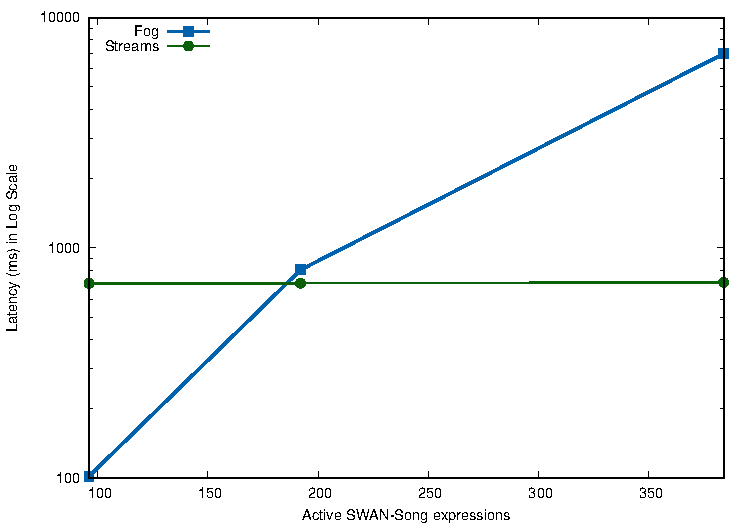
\includegraphics[width=1\textwidth]{images/1_0.pdf}
 \caption{SWAN-Song expressions evaluation with sensors that produce a fresh data record every second. The expressions have the MEAN history reduction mode set and a time window of 5 seconds.}
\label{fig:1_0}
\end{figure}

 \begin{figure}[h!]
\includegraphics[width=1\textwidth]{images/2_0.pdf}
 \caption{SWAN-Song expressions evaluation with sensors that produce a fresh data record every 2 seconds. The expressions have the MEAN history reduction mode set and a time window of 5 seconds.}
\label{fig:2_0}
\end{figure}

\newpage

 \begin{figure}[h!]
\includegraphics[width=1\textwidth]{images/5_0.pdf}
 \caption{SWAN-Song expressions evaluation with sensors that produce a fresh data record every 5 seconds. The expressions have the MEAN history reduction mode set and a time window of 10 seconds.}
\label{fig:5_0}
\end{figure}


The SWAN-Song expressions evaluated over the Fog layer, instead, have a very low latency (less than 35 milliseconds). This performance is achieved because the sensing and the expression evaluations are distributed over different computing nodes. 

The expressions evaluated in the Streams layer have a certain overhead due the data transmission and communication required between the Fog and the Streams layer through the Kafka broker. %In this particular, in this deployment scenario we have a latency of 700 milliseconds. 

\subsection{Sensing Frequency Tests}
In these tests, we offload a certain number of SWAN-Song expressions characterized by different sensing frequencies.
\paragraph{}
Figure \ref{fig:0_5} shows how the Hybrid-Cowbirds reacts when different loads of SWAN-Song expressions are offloaded to the system. The evaluated expressions use a sensor that produces a new data record every 500 ms and have a history window size of 5 seconds. The evaluation has been done in both the Fog and the Streams layer using the core evaluation implementation. 

Increasing the number of active SWAN-Song expressions in the system drastically boosts the latency when the evaluation is performed entirely in the Fog layer. In fact, many active sensors that produce fresh data records with a high-frequency slow down the SWAN-Song expression evaluations. Active threads that simultaneously need (finite) computing resources for fetching new data records or for computing SWAN-Song expressions have to wait for their turn to access the CPU. Furthermore, each sensor thread has to report the sensed data to an expression evaluation thread. Such communication requires synchronization between the sensing and evaluation threads that introduces a certain overhead.
% In particular, sensor threads require mutual exclusion access 
Hence, extra latency is involved with the increase of many concurrent active sensor threads. 

Offloading the same load of SWAN-Song expressions to the Streams layer leads to way better performance. In fact, even though the number of sensing threads per Cowbird Node increases, each produced value is asynchronously sent through the network to the Streams layer. The Streams layer is capable of evaluating 384 active SWAN-Song expressions with a latency of $\sim$700 milliseconds. 

% However, we noticed a decrease in the system performance when the whole system is executed over a long period of time. The reason for this could be the limited resources assigned to the Kafka cluster. In fact, the Kafka cluster acts as a bottleneck in the architecture. We believe that scaling out the Kafka cluster will let the system to achieve better performance. 

\paragraph{}
Figure \ref{fig:1_0} shows how the system performed with SWAN-Song expressions that use sound sensors that produce data with a lower frequency than the previous test case (i.e. new data record every 1 second). For a better understanding of the plotted data, Figure \ref{fig:1_0} reports the achieved results in logarithmic scale.

In this experimental scenario, the Fog performs relatively better than the Streams layer up to a certain threshold of workload. A lower sensor frequency allows the Fog to be more flexible and efficient in comparison to the previous scenario. Figure \ref{fig:2_0} and \ref{fig:5_0} show that even lower frequency (a new date record  every 2 and 5 seconds respectively) sensors reduce latency required to produce an evaluation result in the Fog layer. 
\paragraph{}
We can conclude that with very high-frequency sensors the SWAN-Song evaluation could be offloaded to the Streams layer even though it involves extra communication overheads. By offloading the evaluation to the Streams layer, the Fog layer can be used exclusively to sense sensor data. However, from Figure \ref{fig:1_0} and Figure  \ref{fig:5_0} we can notice that it also makes sense to offload the expressions evaluation to the Streams layer when the number of active sensor threads drastically increases. 

%Figure \ref{fig:5_0} shows that with a high number of active threads the latency increases in the Streams layer even if the offloaded expressions have a low frequency. As already mentioned, one possible explanation can be that the Kafka cluster runs on a single instance node and this could slow down the flow of the whole system.
% We can also notice that in this test the Streams layer performs better than previous scenarios with sensors that generate data with higher frequency. In this case, the Fog layer publish sensors data to the Streams layer with less frequency reducing the Kafka overhead.

\subsection{Scalability Test}
Figure \ref{fig:5_0_3_nodes} shows the results obtained on deploying the SWAN-Song expressions that use sound sensors that produce a new data record every 5 seconds. The evaluation is performed over a time window of 10 seconds. In this test, we deployed the Fog layer with only 5 nodes. We can see that the Fog layer performs worse than what is shown in Figure \ref{fig:5_0} with the same workload. Cowbird Nodes can be added at run time to \emph{scale out} the Fog layer and accommodate bigger loads of data sensing and evaluation.

 \begin{figure}[h!]
\includegraphics[width=1\textwidth]{images/5_0_3_node.pdf}
 \caption{SWAN-Song expressions evaluation with sensors that produce a fresh data record every 5 seconds over a time window of 10 seconds. The Fog layer uses 5 computing nodes (3 Cowbirds Nodes).}
\label{fig:5_0_3_nodes}
\end{figure}


 \begin{figure}[h!]
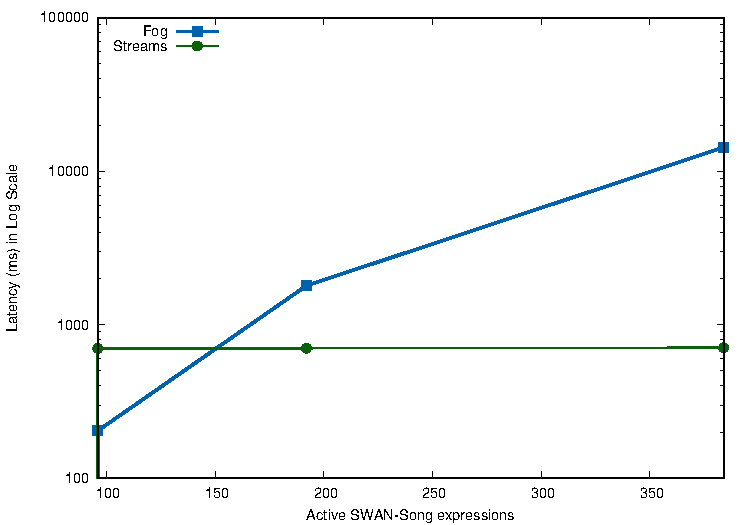
\includegraphics[width=1\textwidth]{images/2_expressions.pdf}
 \caption{SWAN-Song expressions evaluation with two sensors that produce a fresh data record every second over a time window of 5 seconds.}
\label{fig:2_sensors}
\end{figure}

\subsection{Two Sensors Expressions}
We also tested our Hybrid-Cowbirds framework with more complex SWAN-Song expressions. Figure \ref{fig:2_sensors} reports the latency obtained when the system evaluates SWAN-Song expressions composed by two different sensors. For clarity, Figure \ref{fig:2_sensors} reports the achieved latency using logarithmic scale on the y-axis. 

In this experiment, we combined in a SWAN-Song expression the sound sensor with a light sensor that provides information regarding the intensity of the light for a certain area. We designed the expression in order to detect quiet and bright areas. Such an expression is very similar to the SWAN-Song below:
\begin{equation}\label{eq:sound_light_sensor_tristate}
self@sound:value\big\{MEAN, 5000\big\} < 55.0  \text{ \&\& } self@light:value\big\{MEAN, 5000\big\}  > 220.0
\end{equation}

We offloaded the SWAN-Song expression (\ref{eq:sound_light_sensor_tristate}) on our hybrid architecture setting the sensor frequency to a data record per second and the history window to 5 seconds. From Figure \ref{fig:2_sensors} we can notice that the latency obtained by the Fog layer is much higher than what is shown in Figure \ref{fig:1_0}. In both the test cases the sensors data are generated with the same frequency but in this second experiment each expression evaluation has to allocate two different sensing threads.

From Figure \ref{fig:2_sensors} we can also notice that the evaluation in the Streams layer, instead, remains pretty similar to the latency depicted in \ref{fig:1_0}. With up to 384 SWAN-Song expressions the latency of the Streams layer does not encounter any break down.

%\begin{dmath} \label{eq:her}
%self@sound:value\big\{MEAN, 5000\big\} < 55.0 
% 	\text{ \&\& }
% self@light:value\big\{MEAN, 5000\big\}  > 220.0
%\end{dmath}

\subsection{Streaming-Oriented vs Core Implementation}
We performed tests with both the SWAN-Song evaluation strategies implemented for the Streams layer: the \emph{streaming-oriented} and the \emph{core} implementation. As outlined in Chapter 5, the streaming implementation does not keep all the data records generated by sensors but instead it stores only the partial result for each SWAN-Song expression. 

\subsubsection{Streaming-Oriented Storage Efficiency}
We tested the two implementations evaluating sound sensors data with the SWAN MEDIAN history reduction mode over a history window of one hour. Figure \ref{fig:memory_consumption} shows the size of the RocksDB checkpoint directory used by Apache Flink in the Streams layer. Flink periodically records the \emph{state} of the streaming it handles for fault tolerance purposes. After one hour of execution we can notice that the size of the directory used by the \emph{streaming-oriented} evaluation implementation is $\sim$20 times smaller. This can be a good indication of the storage efficiency achieved by the streaming-oriented evaluation implementation.

 \begin{figure}[h!]
\includegraphics[width=1\textwidth]{images/memory_consumption.pdf}
 \caption{RocksDB checkpoint directory size after one hour evaluation of 768 SWAN-Song expressions that use a sound sensor that produces a data  record every second.}
\label{fig:memory_consumption}
\end{figure}

\subsubsection{Evaluating a Large Number of SWAN-Song Expressions in Cowbird Streams}
We also measured the latency with a very high number of active SWAN-Song expressions evaluated in the Streams layer. Figure \ref{fig:1_0_median} shows a comparison of the latency measured with up to 5,000 SWAN-Song expressions deployed on the Cowbird Streams layer. In this scenario, over a test period of 1 hour each Cowbird Node transmitted over the network $\sim$1.5 GB. The evaluations are performed using both the \emph{streaming-oriented} and the \emph{core} implementation. The expressions use sensor threads that generate new data values every 1 second and have a history window of 5 seconds. We can notice that the two implementations react similarly in terms of latency. However, with a high load of expressions the streaming-oriented implementation seems to perform slightly better than the core evaluation strategy. One possible explanation could be a better streaming state management of the streaming-oriented evaluation strategy. As we have seen the streaming-oriented evaluation optimizes space consumption. Hence, when a result is computed only the partial result has to be decompressed from the RocksDB state backend. Instead, using the  core implementation all the data values involved in the evaluation have to be compressed/decompressed from the state backend. Furthermore, the core evaluation generates more communication traffic within the system. In the core evaluation strategy, expression results are computed continuously as fresh data enter the system. Instead, the streaming-oriented implementation uses \emph{fixed} or \emph{aligned} window mechanisms. 

In this test scenario, we achieved a \emph{throughput} of 5,000 events/s with a latency of $\sim$1.1 seconds. When offloading more than 5,000 expressions we noticed delays in the SWAN-Song expressions evaluation. In particular, we experienced a high CPU usage and a slow down of the outbound network traffic. This leads to an increment of the size of the outgoing message buffers and then to a bigger heap consumption. We also observed a decrease of the Kafka broker performance because of the active traffic between the Fog and the Streams layer. This is a clear symptom that the Fog layer should be scaled-out along with the Kafka instance. 
 \begin{figure}[h!]
\includegraphics[width=1\textwidth]{images/1f_MEDIAN.pdf}
 \caption{SWAN-Song expressions evaluation with sensors that produce a fresh data record every second. The expressions have the MEDIAN history reduction mode set and a time window of 5 seconds.}
\label{fig:1_0_median}
\end{figure}


\section{Discussion}
In this section we described some of the tests we performed on our Hybrid-Cowbirds architecture. From the results of our experiments emerge that in some scenarios it makes sense to combine the data sensing and  the SWAN-Song evaluation in the Fog layer. As we have seen in the \emph{Scalability Test} described in Subsection 6.4.3, the Fog layer can scale out easily in order to accommodate an increasing number of SWAN-Song expression evaluation requests. However, experimental results outlined in Subsection 6.4.2 highlight that after a certain threshold, the Fog layer cannot handle anymore the burden of evaluating the sensed data in scenarios characterized by \emph{high-frequency} sensors.
% However, according to the results obtained from our \emph{Sensing Frequency Tests} is that in situations characterized by \emph{high-frequency} sensors the Fog layer cannot handle anymore the burden of evaluating the sensed data. In these contexts, the evaluation can be simply offloaded to the Streams layer. 
The Streams layer along with the sensing capabilities provided by the Fog layer can guarantee real-time performance for data evaluations.

Furthermore, not only SWAN-Song expressions characterized by high-frequency sensors can be offloaded to the Streams layer. Some applications require sensor data collected over long time windows such as hours or even days. Such scenarios could certainly benefit from the Streams layer. In the original design of the SWAN framework, all the sensor values are kept in memory. Hence, the memory heap could be easily saturated if many long-running SWAN-Song expressions are allocated. %As a matter of fact, with 64 active sound sensor threads that produce a float data value every second the Java default heap size is saturated in less than 2hrs u .

Long-running SWAN-Expressions could be offloaded to the Streams layer that runs on a cluster that is usually characterized by Terabyte of memory and Petabyte of disk.  

\paragraph{}
The Kafka broker is the backbone of the Hybrid-Cowbirds architecture. In actual deployment, it should be characterized by multiple nodes and it should scale-out along with the Fog layer in order to prevent it from becoming a communication bottleneck between the Fog and the Streams layer as happened in our \emph{Evaluating a Large Number of SWAN-Song Expressions in Cowbird Streams} test (Subsection 6.4.5). 

\paragraph{}
We tested the \emph{streaming-oriented} evaluation realized for the Streams layer in our \emph{Streaming-Oriented vs Core Implementation} tests (Subsection 6.4.5). We demonstrated that it is more efficient than the core implementation when storing the data streaming state. This could bring benefits when evaluating long-running expressions characterized by a relatively big internal streaming state.

\paragraph{}
In a Fog computing context, the tested setup is not very realistic. In fact, all the architecture components run in the same SURFsara data center. As already mentioned in Chapter 5, the architecture could be geographically distributed putting the Fog layer closer to the user. In such scenario, sensor evaluation capabilities will be close to the data generation and to the users. This approach makes possible the definition of a general purpose platform for evaluating smartphone and IoT sensors that would be ready to meet the Fog computing concept. Such a platform would be indeed characterized by low latency and high availability.
\clearpage{\pagestyle{empty}\cleardoublepage}
\chapter{Related work}
The internet traffic explosion started in the mid-90s induced the creation of massive datasets. Processing very large amount of data, even though can be conceptually straightforward, actually means many computations that have to be distributed across hundreds or thousands of machines in order to finish in a reasonable amount of time. In early 2000s, the developer had the burden to write complex applications responsible for parallelizing the computation, distributing the data, and handling possible failures. As a reaction to this complexity, Google in 2004 published a paper describing a novel programming model for processing large datasets named MapReduce \cite{googlemapreduce}. MapReduce provides an abstraction that allows the developer to focus on the computation he/she wants to express hiding the details of parallelization, fault-tolerance, data distribution and load balancing in a framework. The MapReduce framework takes advantage of the Google File System \cite{googlefilesystem}: a distributed file system that uses replication to provide availability and reliability on top of commodity unreliable hardware. The open source community, inspired by the Google MapReduce programming model, created Hadoop \cite{hadooponline} and HDFS \cite{hadoophdfs}. The Hadoop release boosted the growth of the big data analysis field and created new scenarios and new type of applications that were very tough to realize with previous existing tools. From that moment on, a lot of effort has been put in realizing more efficient and high-performance technologies for collecting, aggregating and analyzing huge amount of data.

In this chapter we will discuss some of the technologies and architectures that can be used in order to process large amount of data generated by (IoT) sensors, possibly in real-time.

\section{Batch-Mode architecture}
Google MapReduce and Hadoop are designed to be executed on top of clusters of computing nodes. The first releases of Hadoop integrated the cluster resource management with the data processing engine itself (Hadoop MapReduce). In 2012, Hadoop 2.0 was released \cite{hadooponline} and it introduced YARN \cite{yarn}; Apache Yet Another Resource Negotiator (YARN) decouples the programming model from the resource management infrastructure and the users' applications scheduling. In general, we can think to YARN as a distributed operating system that is capable of managing a cluster of machines and scheduling users' applications on the available resources. Furthermore, it provides an API that can be used to develop any generic distributed application. Hence, different computing frameworks that address different application requirements have been built on top of YARN (e.g. the general purpose Apache Spark \cite{apachesparkonline}, Apache Giraph \cite{apachegiraphonline} for iterative graph processing, etc.). 

 \begin{figure}[ht!]
\includegraphics[width=1\textwidth]{images/barch_architecture.pdf}
 \caption{Classic big data batch architecture}
\label{fig:batch_architecture}
\end{figure}

A big data application usually has a well defined architecture, no matter the computing framework it uses and whether or not it runs on top of YARN or on another cluster management system (e.g. Apache Mesos  \cite{apachemesosonline}, Kubernetes \cite{kubernetesonline}, in the cloud using Amazon Elastic Map Reduce (EMR) \cite{amazonemronline}). The \emph{classic} big data architecture for processing large amount of structured or unstructured data is named \emph{batch architecture} \cite{philosophydistributeddata, fastdataarchitecture, streamingbigdataprocessinginclouds}. The typical big data batch architecture consists of the following components or layers (see Figure \ref{fig:batch_architecture}):
\begin{itemize}
\item	 \emph{Data ingestion layer}. The data ingestion layer can be used to move data that can come from different sources into the persistence tier. The data ingestion layer can take advantage of special-purpose services such as Apache Flume \cite{apacheflumeonline} for log aggregation or Apache Sqoop \cite{apachesqooponline} for interoperating with databases.
\item \emph{Data persistence.} The data persistence layer is responsible of storing and indexing final as well intermediate datasets. This tier can store large amount of data using one of the next-generation database systems. In fact, the Dynamo \cite{dynamo} paper accelerated interest in NoSQL systems and many NoSQL database emerged such as Apache Cassandra \cite{apachecassandraonline} or MongoDB \cite{mongodbonline}. Furthermore, the CAP theorem emerged as a way of understanding the trade-offs between consistency and availability of service in distributed systems when a network partition occurs. For the always-on applications, it often made sense to accept \emph{eventual consistency} in exchange for a greater availability \cite{fastdataarchitecture}. In big data application, database systems are often used when row-level access (e.g. CRUD operations) is required \cite{fastdataarchitecture}.

In order to store large datasets, the data persistence layer can also use a distributed file system or object store, such as HDFS or Amazon S3 \cite{awss3online}. These systems offers lower cost per GB storage compared to databases and more flexibility for data formats \cite{fastdataarchitecture}. However, they are best used when scans are the dominant access pattern, rather than CRUD operations. 
\item  \emph{Cluster resource management}. 
\item  \emph{Data Processing.} The data analysis jobs written in Hadoop MapReduce, Spark, or other tools submitted to the cluster resource manager.
\end{itemize}

A typical big data application can be built as a \emph{workflow}, a directed graph of distributed computing jobs \cite{bigdataatlinkedin}. Each job reads one or more input datasets from the persistent storage and produces one or more output datasets. In MapReduce, if the application requires data reuse between computations (e.g. between two jobs) the intermediate result is also written to an external stable storage system. This can incur substantial overheads due to data replication, disk I/O, and serialization, which can dominate application execution times. Recognizing this problem, researchers have developed specialized frameworks for some applications that require data reuse. These frameworks only support specific computation patterns and perform data sharing implicitly for these patterns. Eventually, the general purpose computing framework Apache Spark \cite{apachespark} was released. Spark is the first system that allows a general-purpose programming language to be used at interactive speeds for in-memory data mining on clusters \cite{apachespark}. Spark is based on the concept of resilient distributed datasets (RDDs) \cite{apachesparkrdd} that enables efficient data reuse in a broad range of applications. The RDD abstraction allows users to explicitly persist intermediate results in memory, control the data partitioning to optimize the data placement, and manipulate them using a rich set of operators. Even though Spark increased the interactivity of many big data applications and tools, a typical job in batch-mode can last from few minutes to several hours. In fact, in classic batch-mode, data is collected and stored in the persistent storage layer and once in a while (e.g. every hour, once per day) the data is processed through one or more batch jobs. The high-latency imposed by the batch architecture is not suitable for real-time applications in which data should be computed as it is generated, in an incremental fashion.

\section{Real-time streaming architecture}
Recently, many big data real-time applications emerged such as detecting fraudulent financial activity as it happens or optimizing e-commerce search results in real-time. These kinds of applications process unbounded datasets and potentially infinite \emph{streams} of data, and they are often  referred as real-time streaming applications. The backbone of a real-time streaming application is usually a distributed, high-performance and always available architecture. There are many streaming systems and ways of doing streaming, and everything is evolving quickly. In this section, we will discuss and highlight the components required to build an efficient streaming architecture.




\clearpage{\pagestyle{empty}\cleardoublepage}
\chapter{Conclusions and Future Work}
\section{Conclusions}
We designed and implemented a distributed architecture for the Cowbird framework. The distributed architecture promotes the sensing and evaluation of streams of sensor data in real-time. The architecture is composed by a distributed and scalable sensing layer and by a stream processing platform that is capable of evaluating large loads of SWAN-Song expressions with a low latency. Furthermore, when it is possible, the system combines sensing and evaluation features in the Fog layer avoiding extra communication costs. The architecture is extremely versatile and both its components can easily scale in situations of high input loads.
\paragraph{}
We built an experimental application that monitors the level of noise emitted by IoT sound sensors. This application helped us testing the designed architecture and measures its performance in a relatively simple setup. We conclude that the SWAN-Song expressions evaluation can be performed by both the architectural layers depending by the scenario. SWAN-Song characterized by \emph{high-frequency} sensors or expressions that have a long history time window should be offloaded to the Streams layer. 

\section{Future Work}
As future work, a real-time adaptive heuristic for offloading expression evaluations from the Fog layer to the Streams layer can be developed. This heuristic can be executed by the Remote Evaluation Manager running in the Fog layer with the goal to minimize latency in the SWAN-Song expressions evaluation. This algorithm can also select the most suitable evaluation strategy: \emph{core} or \emph{streaming-oriented}. To this end, the streaming-oriented evaluation implementation could be realized also for the Fog layer.
\paragraph{}
The feasibility of adopting the realized architecture in a fog computing scenarios should be investigated as well. In fact, the Fog layer of our hybrid architecture could be deployed on the \emph{edge} while the Streams could be executed in a cloud environment.
\paragraph{}
In addition, Cowbird Node internal components can be re-engineered as Akka actors instead of native Java threads. The Akka actor model could be used not only for handling communication between different nodes but also for threads management in the Cowbird Node instance. This approach could reduce synchronization overheads between sensors threads and expressions evaluation mechanisms. In fact, the communication between actors happens through asynchronous exchanged messages. Moreover, Akka maps running actors to a pool of active threads. Hence, resource utilization could be improved when many active sensors threads are allocated.
\paragraph{}
As a further improvement, sensed and evaluated data in the cloud could be shared among different SWAN users that require the same type of sensor data. Sharing sensed and derived sensor data would enhance resource utilization avoiding storage and computing workload duplication.
\paragraph{}
In order to increase performance and efficiency in the communication between the Fog and the Streams layer, a message binary format could be used instead of JSON.
\paragraph{}
Another possible improvement can be extending the SWAN-Song semantics to make it benefit from the capabilities brought by Apache Flink. Apache Flink has a vast ecosystem of libraries such as Complex Event Processing (CEP) \cite{flinkceponline} or machine learning \cite{flinkmlonline}. SWAN-Song can be enriched with these features in order to offer a more rich API to mobile developers that want to use sensors data in their apps. 





 
\clearpage{\pagestyle{empty}\cleardoublepage}
%\include{Architettura}
%\clearpage{\pagestyle{empty}\cleardoublepage}
%\include{TED}
%\clearpage{\pagestyle{empty}\cleardoublepage}
%!TEX encoding = UTF-8 Unicode\pagestyle{empty}
%\clearpage{\pagestyle{empty}\cleardoublepage}
%\include{APIs}
%\clearpage{\pagestyle{empty}\cleardoublepage}
%\include{Test}
%\clearpage{\pagestyle{empty}\cleardoublepage}


%%%%%%%%%%%%%%%%%%%%%%%%%%%%%%%%%%%%%%%%%non numera l'ultima pagina sinistra
\clearpage{\pagestyle{empty}\cleardoublepage}
%%%%%%%%%%%%%%%%%%%%%%%%%%%%%%%%%%%%%%%%%per fare le conclusioni

%\chapter*{Conclusions and Future Work}
%%%%%%%%%%%%%%%%%%%%%%%%%%%%%%%%%%%%%%%%%imposta l'intestazione di pagina
%\rhead[\fancyplain{}{\bfseries
%CONCLUSIONI}]{\fancyplain{}{\bfseries\thepage}}
%\lhead[\fancyplain{}{\bfseries\thepage}]{\fancyplain{}{\bfseries
%CONCLUSIONI}}
%%%%%%%%%%%%%%%%%%%%%%%%%%%%%%%%%%%%%%%%%aggiunge la voce Conclusioni
                                        %   nell'indice
%\addcontentsline{toc}{chapter}{Conclusioni e sviluppi futuri} 
%\input{ConclusionAndFutureWorks}

 % Latency (ms) in Log scale 
 
 %\cite{K3,K4}.
%%%%%%%%%%%%%%%%%%%%%%%%%%%%%%%%%%%%%%%%%imposta l'intestazione di pagina
%\renewcommand{\chaptermark}[1]{\markright{\thechapter \ #1}{}}
%\lhead[\fancyplain{}{\bfseries\thepage}]{\fancyplain{}{\bfseries\rightmark}}
%\appendix                               %imposta le appendici
%\chapter{Configurazioni utilizzate nei test}               %crea l'appendice


%%%%%%%%%%%%%%%%%%%%%%%%%%%%%%%%%%%%%%%%%non numera l'ultima pagina sinistra
\printbibliography 
\clearpage{\pagestyle{empty}\cleardoublepage}
\chapter*{Acknowledgement}
I would like to say thank you to my supervisors Henri and Roshan. Thank you for the advice you gave me during these months! Because of you I learned a little bit more of what doing research actually means. It has been an incredible experience working with you. Furthermore, I would like also express my gratitude to Kees for the valuable feedback he gave me during the thesis writing.

\paragraph{}
I would like to say thank you to my mom, dad, Kevin and Ludovica for all the support they gave me in the past two years. You always believed in me and you constantly gave me the strength to push forward throughout my studies. Thank you for supporting me in every choice I made. I will always be grateful for what you did for me.

\paragraph{}
Thank you.
\end{document}
